
\section{Convolutional Autoencoder}\label{sec:convae_implement}

The convolutional autoencoder class \lstinline{ConVae} is implemented as a subclass of \lstinline{LatentModel}. It implements the construction of the computational graph and the compute operations needed for the possible losses. To ascertain that the graph is constructed before the loss is computed, the user never interfaces with the \lstinline{_ModelGraph} and \lstinline{_ModelLoss} methods that implement the respective functionalities. Instead, the user calls a wrapper method from the parent class \lstinline{LatentModel.compile_model}, which compiles the model for training.

The graph is constructed with specifications from configuration dictionaries passed through the \lstinline{compile_model} method. The first of which specifies the activation function as well as the strength, and type of, weight regularization. The second dictionary specifies the type of reconstruction loss used in the optimization.

\subsection{Computational graph}

The private\footnote{The term private is used loosely in the context of \lstinline{python} programs, as the language does not actually maintain private methods. However, methods that are prefixed with an underscore are to be treated as private and are not exposed with public APIs and in documentation by convention.} function which enacts the computational graph is \lstinline{_ModelGraph}. It accepts arguments for the strength and type of regularization on the kernel and bias parameters as well as the activation function to be used for the internal representations, and the projection to output space. 

The encoder is constructed with a for loop over the number of layers, using a 2D convolutional layer and best practices for the application of batch-normalization. Wherein the normalization is applied after the activation for exploding-gradient susceptible functions and before for functions with a vanishing gradient problem. In TensorFlow, we implement the construction of the encoder as 

\begin{lstlisting}[language=iPython]
# excerpt from convolutional_VAE.py
# at https://github.com/ATTPC/VAE-event-classification
# from commit ca9b722
kernel_reg=reg.l2
kernel_reg_strength=0.01
bias_reg=reg.l2
bias_reg_strenght=0.00
activation="relu"
output_activation="sigmoid"

activations = {
    "relu": tf.keras.layers.ReLU(),
    "lrelu": tf.keras.layers.LeakyReLU(0.1),
    "tanh": Lambda(tf.keras.activations.tanh),
    "sigmoid": Lambda(tf.keras.activations.sigmoid),
}

self.x = tf.keras.layers.Input(shape=(self.n_input,))
# self.x = tf.placeholder(tf.float32, shape=(None, self.n_input))
self.batch_size = tf.shape(self.x)[0]
self.x_img = tf.keras.layers.Reshape((self.H, self.W, self.ch))(self.x)
h1 = self.x_img  # h1 = self.x_img
shape = K.int_shape(h1)

k_reg = kernel_reg(kernel_reg_strength)
b_reg = bias_reg(bias_reg_strenght)
# ... code omitted for brevity
for i in range(self.n_layers):
                with tf.name_scope("conv_" + str(i)):
                    filters = self.filter_arcitecture[i]
                    kernel_size = self.kernel_architecture[i]
                    strides = self.strides_architecture[i]
                    if i == 0 and pow_2:
                        padding = "valid"
                    else:
                        padding = "same"

                    h1 = Conv2D(
                        filters,
                        (kernel_size, kernel_size),
                        strides=(strides, strides),
                        padding=padding,
                        use_bias=True,
                        kernel_regularizer=k_reg,
                        # bias_regularizer=b_reg
                    )(h1)

                    if activation == None:
                        pass
                    elif activation == "relu" or activation == "lrelu":
                        a = activations[activation]
                        h1 = a(h1)
                        with tf.name_scope("batch_norm"):
                            if self.batchnorm:
                                h1 = BatchNormalization(
                                    axis=-1,
                                    center=True,
                                    scale=True,
                                    epsilon=1e-4
                                )(h1)
                                self.variable_summary(h1)
                    else:
                        a = activations[activation]
                        with tf.name_scope("batch_norm"):
                            if self.batchnorm:
                                h1 = BatchNormalization(
                                    axis=-1,
                                    center=True,
                                    scale=True,
                                    epsilon=1e-4
                                )(h1)
                                self.variable_summary(h1)
                        h1 = a(h1)

                    if self.pooling_architecture[i]:
                        h1 = tf.layers.max_pooling2d(h1, 2, 2)

\end{lstlisting}

Inside the method the placeholder variable \lstinline{ConVae.x} is defined. The placeholder defines the entry point of the forward pass and is where TensorFlow allocates the batched data when optimizing and making predictions. Depending on whether the model is instructed to use the VGG16 representation of the data or a specified encoder structure it applies dense weight transformations with non-linearities or computes a series of convolutions respectively. Each convolutional layer is specified with a kernel size, a certain number of filters, and the striding. We also use a trick from \citet{Guo2017} to determine the padding size, ensuring that the padding is chosen such that the reconstruction size is unambiguous. The padding is set to preserve the input dimensionality and is only reduced in dimensionality with striding or max-pooling. If the input dimension is of size $2^n$, where $n$ is the number of layers, the last convolution is adjusted to have no zero-padding. 

After each layer, the specified non-linearity is applied. The models accept one of the sigmoid activations (logistic sigmoid or hyperbolic tangent) or the rectified linear unit family of functions as activations\footnote{The model accepts a \lstinline{None} argument for the activation in practice for debugging but this is not used for any models in this thesis.}. If the model configuration specifies to use batch normalization, this is applied before sigmoid functions and after rectified units. The reason for different points of application relates to the challenges of the respective activation families; sigmoids' saturate and so the input should be scaled, and rectified units are not bounded so the output is scaled. The output from the encoder is then a tensor with dimensions \lstinline{h = (o, o, f)} where \lstinline{f} is the number of filters in the last layer and \lstinline{o} $= \frac{H}{2^n}$ where $n$ denotes the number of layers with stride $2$ or the count of \lstinline{MaxPool} layers, and $H$ gives the input image size.

The tensor output from the encoder is then transformed to the latent space with either a simple dense transformation, e.g. \lstinline{z = Dense(flatten(h))}. Alternatively, if a variational loss is specified, a pair mean and variance tensors. These are constructed with dense transformations from \lstinline{h}. The mean and variance tensors are then stored as class attributes of the ConVae instance:

\begin{lstlisting}[language=iPython]
self.mean = Dense(self.latent_dim, kernel_regularizer=k_reg)(h1)
self.var = Dense(self.latent_dim, kernel_regularizer=k_reg)(h1)
\end{lstlisting}

 Using the re-parametrization trick shown by \citet{Kingma2013}, we introduce stochasticity to the sample tensor in a manner which allows training by backpropagation. With re-parametrization, the sample is generated as \lstinline{z = self.mean + tf.exp(self.var)*epsilon}, where epsilon is a stochastic tensor from the multivariate uniform normal distribution $\mathcal{N}(0, 1)$. Note that the \lstinline{self.var} is treated as the log of the variance. Furthermore, he mean and standard deviation tensors are stored as class attributes to be used in the computation of the loss. The latent sample is also set as a class attribute for prediction.

After a sample \lstinline{z} is drawn, the decoder computes the reconstruction for a given sample. The decoder is configured according to the instructions supplied in the initialization of the algorithm. In the case that the inputs are from a pre-trained model representation the model has the same call structure but with a boolean flag to the model \lstinline{use_vgg} that indicates that the configuration is explicitly for the decoder. 

\subsection{Computing losses}

To compute the loss(es) the \lstinline{ConVae} implements the second of \lstinline{LatentModel}s abstract methods; \lstinline{_ModelLoss}. Like the graph construction, this method is never called directly but through the interface of the parent class in the \lstinline{LatentModel.compile_model} method.  In a similar vein, losses are configured using a supplied dictionary.

The reconstruction loss is specified in the configuration dictionary, and the model accepts either a mean squared error or binary cross-entropy loss with cross-entropy as the default. Each of these losses acts pixel-wise on the output and target images. When computed, the construction loss is stored as a class attribute, \lstinline{ConVae.Lx}, which is logged to a \lstinline{TensorBoard}\footnote{This is a module for tracking the progress of a model during training. It supports visualizations as well as automatically plotting the model graph, etc.} instance. The reconstruction loss is then implemented as


\begin{minipage}{\linewidth}
\begin{lstlisting}[language=iPython]
# excerpt from convolutional_VAE.py
# at https://github.com/ATTPC/VAE-event-classification
# from commit ca9b722
x_recons = self.output
if self.use_vgg:
    self.target = tf.placeholder(tf.float32)
else:
    self.target = self.x
if reconst_loss == None:
    reconst_loss = self.binary_crossentropy
    self.Lx = tf.reduce_mean(
        tf.reduce_sum(reconst_loss(self.target, x_recons), 1)
    )
elif reconst_loss == "mse":
    self.Lx = tf.losses.mean_squared_error(self.target, x_recons)
\end{lstlisting}
\end{minipage}


Depending on the configuration, the model then compiles a loss over the latent space. In a variational autoencoder, the loss is a  Kullback-Leibler divergence (KL-divergence) of the latent distribution with a multivariate normal distribution with zero mean and unit variance. This has a closed-form solution given a tensor representing the mean and standard deviation, which we derived in equation \ref{eq:kl_opt}. This equation is relatively straightforward to implement, as it just implies a sum over the mean and log-variance tensor. The form of equation \ref{eq:kl_opt} also makes clear why we parametrize the log-variance and not the variance directly as the exponentiation ensures positivity of the variance.


\begin{minipage}{\linewidth}
\begin{lstlisting}[language=iPython]
def kl_loss(self, args):
    """
    kl loss to isotropic zero mean unit variance gaussian
    """
    mean, var = args
    kl_loss = -0.5 * K.sum(
        1 + self.var - K.square(self.mean) - K.exp(self.var), axis=-1
    )
    return tf.reduce_mean(kl_loss, keepdims=True)
\end{lstlisting}
\end{minipage}

Alternatively to a KL-divergence the latent space may be regularized in the style proposed by \citet{Zhao}. In this paradigm we compute a loss over the entire latent sample, and not component wise as the KL-divergence does. We use the radial basis function kernel to compute the maximum mean discrepancy divergence term introduced in equation \ref{eq:mmd}, and use the implementation provided by \cite{Zhao} on their \href{http://szhao.me/2017/06/10/a-tutorial-on-mmd-variational-autoencoders.html}{website}. We choose the prior distribution fore MMD divergence to be a Gaussian mixture of two normal distributions with unit variance and means with a distance $\geq 3\sigma$ from each other. 

\subsection{Applying the framework}

To illustrate the use and functionality of the model we'll demonstrate the pipeline for constructing a semi-supervised and clustering version of the architecture using the code written for this thesis. Beginning with the semi-supervised use-case. These tutorials are also available in the Github repository for the thesis. They are provided as \lstinline{jupyter-notebooks} and can be viewed in browser, or hosted locally. The example takes the reader through the entirety of the analysis pipeline as presented in chapter \ref{ch:architectures} and shows how the model was fit to data as well as post-analysis steps. 

The goal of this example is to introduce the reader to the analysis framework used in this thesis. We will go through defining a model with convolutional parameters and fit this model to simulated AT-TPC events. With a 2D latent space this allows us to explore the latent configuration directly, but yields worse reconstructions. The \href{https://github.com/ATTPC/VAE-event-classification/blob/master/notebooks/simulated_tutorial.ipynb}{notebook-tutorial} walks through the example and is entirely analogous to this section.

We begin by loading the data files. The repository comes equipped with a small data-set of simulated data that can be analyzed. To achieve reasonable run-times a GPU enabled TensorFlow distribution is encouraged\footnote{If the run-time is too slow the data can be replaced with the MNIST data, which is much smaller in terms of size per data-point}. We assume that the script as we walk through it is located in the \lstinline{notebooks/} directory of the repository. We begin by making the necessary imports for the analysis. The packages \lstinline{TensorFlow} and \lstinline{matplotlib} have to be installed on the system for the tools to work, along with \lstinline{Numpy} and \lstinline{pandas}. The \lstinline{data_loader} module contains functions to load files to \lstinline{numpy} arrays, while the module \lstinline{convolutional_VAE} contains the model class itself.

\begin{minipage}{\linewidth}
\begin{lstlisting}[language=iPython]
import sys
sys.path.append("../src/")
import matplotlib.pyplot as plt
import tensorflow as tf
import data_loader as dl
from convolutional_VAE import ConVae
\end{lstlisting}
\end{minipage}

\noindent Next the simulated data has to be loaded into memory, and we display four events to illustrate what the representation of the data  looks like.  

\begin{minipage}{\linewidth}
\begin{lstlisting}[language=iPython]
x_full, x_labelled, y = dl.load_simulated("128")

fig, axs = plt.subplots(ncols=4, figsize=(14, 5))
[axs[i].imshow(x_full[i].reshape((128, 128)), cmap="Greys") for i in range(4)]
[axs[i].axis("off") for i in range(4)]
plt.show()
\end{lstlisting}
\end{minipage}

\begin{figure}[H]
\centering
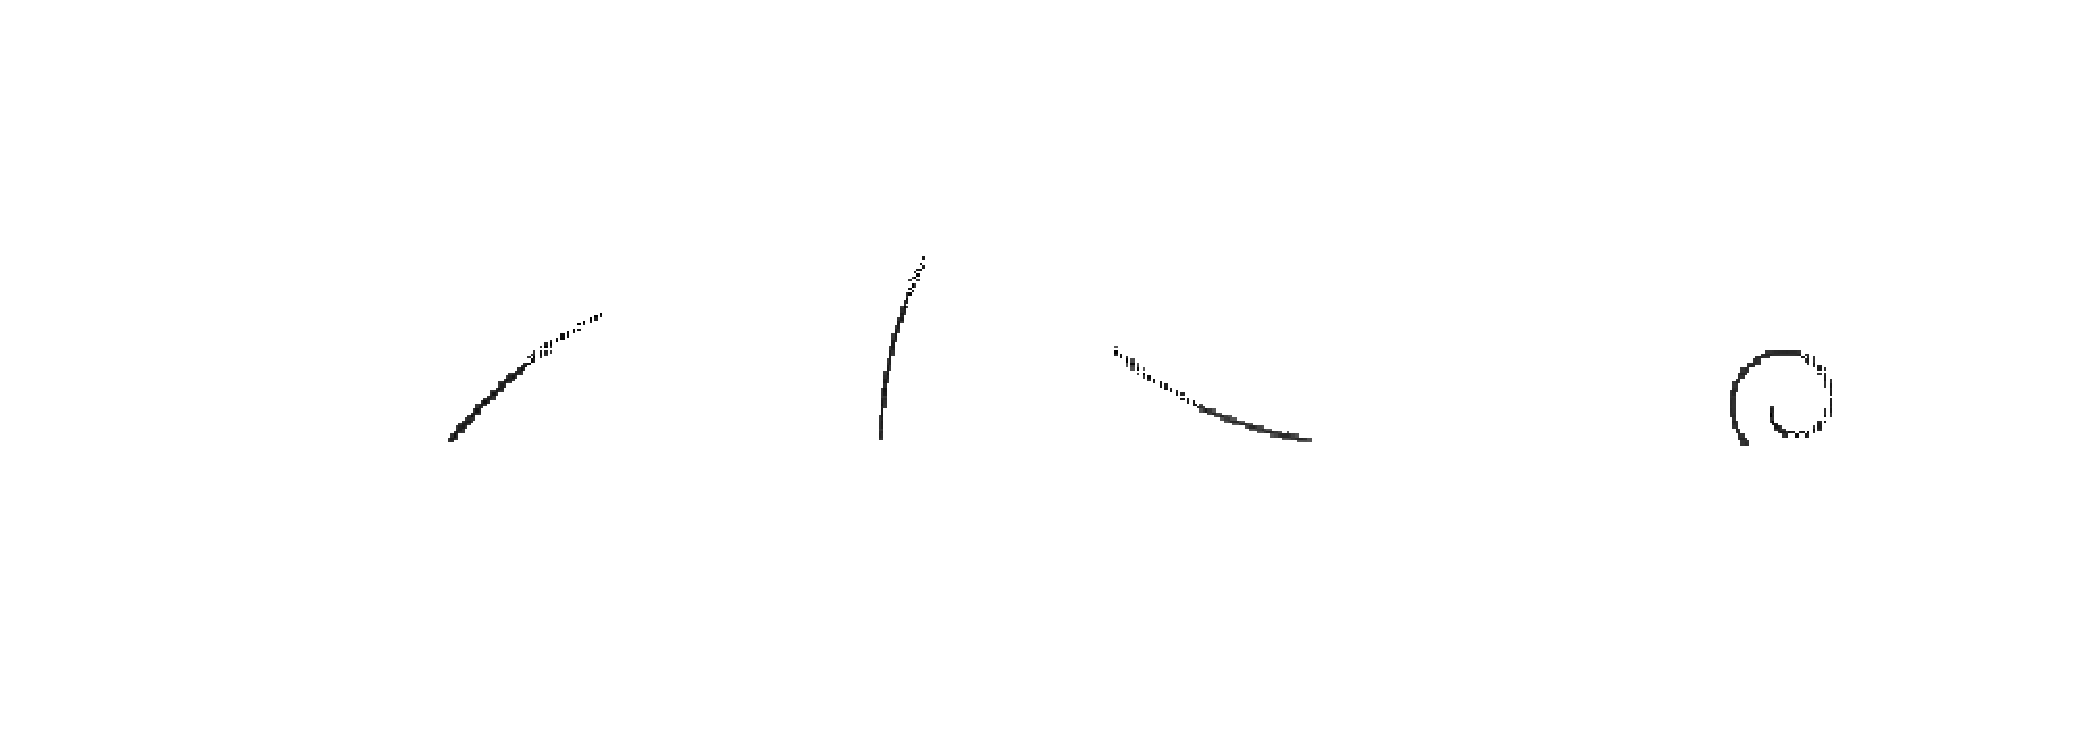
\includegraphics[width=\textwidth]{sim_events.pdf}
\caption[simulated events]{Selection of four simulated events in their XY-projection used as targets to reconstruct with the convolutional autoencoder.}\label{fig:sim_data}
\end{figure}

\noindent We are now ready to define our model. To instantiate the model a convolutional architecture needs to be specified, in our implementation these are supplied as lists of integers, and a single integer specifying the number of layers. We'll use four convolutional layers and the simplest mode-configuration that uses no regularization on the latent space.  

\begin{minipage}{\linewidth}
\begin{lstlisting}[language=iPython]
n_layers = 4
kernel_architecture = [5, 5, 3, 3]
filter_architecture = [8, 16, 32, 64]
strides_architecture = [2, 2, 2, 2]
pooling_architecture = [0, 0, 0, 0]

mode_config = {
    "simulated_mode":False, #deprecated, to be removed
    "restore_mode":False, #indicates whether to load weights 
    "include_KL":False, #whether to compute the KL loss over the latent space
    "include_MMD":False, #same as above, but for the MMD loss
    "include_KM":False, #same as above, but K-means. See thesis for a more in-depth treatment of these
    "batchnorm":True, #whether to include batch-normalization between layers
    "use_vgg":False, #whether the input data is from a pre-trained model 
    "use_dd":False, #whether to use the duelling-decoder objective 
}

model = ConVae(
    n_layers,
    filter_architecture,
    kernel_architecture,
    strides_architecture,
    pooling_architecture,
    2, #latent dimension,
    x_full,
    mode_config=mode_config
)
\end{lstlisting}
\end{minipage}


\noindent When the model is defined two steps have to be completed before we train it. Firstly model has to be compiled, which constructs the forward pass and computes the select losses over the outputs from the forward pass. Secondly the gradient-graph has to be computed, as it defines the iterative step for the optimization. For the former the model accepts two dictionaries that specify details of the forward pass; a dictionary \lstinline{graph_kwds} which specifies the activation function and a dictionary \lstinline{loss_kwds} regularization and the type of loss on the reconstruction, be it cross entropy or mean squared error. When the model is compiled it will print to the console a table of its configuration allowing the researcher to confirm that the model is specified correctly. This print is omitted for brevity but can be found in the notebook.


\begin{minipage}{\linewidth}
\begin{lstlisting}[language=iPython]
graph_kwds = {
    "activation": "relu",
    "output_activation": "sigmoid", # applied to the output, necessary for BCE
    "kernel_reg_strength": 1e-5
}
loss_kwds = {
    "reconst_loss": None # None is the default and gives the BCE loss 
}
model.compile_model(graph_kwds, loss_kwds)
\end{lstlisting}
\end{minipage}


\noindent For the latter the model accepts an object of a \lstinline{TensorFlow} optimizer, which should be uninstantiated, and arguments that should be passed to that optimizer object. In this example we choose an adam optimization scheme with $\beta_1 = 0.8$ and $\beta_2=0.99$ and a learning rate of $\eta=\num{1e-3}$. The parameters are explained in detail in section \ref{sec:gd}, but determine the weighting of the first and second moment of the gradient and the size of the change allowed on the parameters respectively. 

\begin{minipage}{\linewidth}
\begin{lstlisting}[language=iPython]
optimizer = tf.train.AdamOptimizer
opt_args = [1e-3, ] #learning rate
opt_kwargs = {"beta1": 0.8, "beta2":0.99}
model.compute_gradients(optimizer, opt_args, opt_kwargs)
\end{lstlisting}
\end{minipage}

\noindent When the model is compiled and the gradients are computed it is ready to be trained, or alternatively a pre-trained model can be loaded into memory. Model training is performed by specifying a number of epochs to run for and the batch size to use for the optimization. Additionally the model takes a \lstinline{TensorFlow} session object which it uses to run parts of the graph including the optimization operations. We also specify that the model should stop before the specified number of epochs with the \lstinline{earlystopping} flag if the model converges or starts to overfit.

\begin{minipage}{\linewidth}
\begin{lstlisting}[language=iPython]
epochs = 200
batch_size = 150
earlystop = True
sess = tf.InteractiveSession()

lx, lz = model.train(
    sess,
    epochs,
    batch_size,
    earlystopping=earlystop
)
\end{lstlisting}
\end{minipage}

\noindent The training prints the value for the reconstruction, $L_x$, and latent $L_z$ losses as well as the evaluation of the early-stopping criteria. This record is omitted for brevity, but can be seen in the notebook. After the model is trained we wish to inspect the reconstructions. Computing the reconstructions is done with the \lstinline{session} object which feeds an input, in this case four events, to the model and retrieves a specific point on the graph. For this example we retrieve the reconstructions defined as the model output; \lstinline{model.output}.

\begin{minipage}{\linewidth}
\begin{lstlisting}[language=iPython]
sample = x_full[:4].reshape((4, -1))
feed_dict = {model.x:sample}
reconstructions = model.sess.run(model.output, feed_dict)
reconstructions = reconstructions.reshape((4, 128, 128))
\end{lstlisting}
\end{minipage}

\noindent We reshape the reconstructions to the image dimension and plot them using the same block of code as we did for showing the original events, only adding another row. 

\begin{minipage}{\linewidth}
\begin{lstlisting}[language=iPython]
fig, axs = plt.subplots(nrows=2, ncols=4, figsize=(14, 5))
[axs[0][i].imshow(x_full[i].reshape((128, 128)), cmap="Greys") for i in range(4)]
[axs[1][i].imshow(reconstructions[i], cmap="Greys") for i in range(4)]
[(axs[0][i].axis("off"), axs[1][i].axis("off")) for i in range(4)]
plt.show()
\end{lstlisting}
\begin{figure}[H]
\centering

\includegraphics[width=0.8\textwidth, height=8cm]{reconst_sim_events.pdf}
\caption[Simulated events and reconstructions]{Showing four events and their corresponding reconstructions. The reconstructions faithfully reconstruct the artifacts from the simulation procedure but has a fuzzy quality common to the ELBO approximation.}\label{fig:reconst_sim}
\end{figure}
\end{minipage}

From figure \ref{fig:reconst_sim} we that while the reconstructions are fuzzy they capture the important parts of the input, notably  the curvature of the proton. What remains now is the exploration and fitting of the latent space. We begin by computing the latent representation of the labelled subset of the data. This is done with the \lstinline{run_large} method which does a computation a few elements at a time as the memory requirements of the computations scale very poorly. The method accept an argument for the session with which to run the required output, what output we wish to retrieve and the input needed to compute that output. In this case we wish to compute the latent representation and so our output is \lstinline{mpdel.z_seq[0]}. To preserve homogeneity with the DRAW implementation the latent sample is stored as an iterable. 

\begin{minipage}{\linewidth}
\begin{lstlisting}[language=iPython]

all_labelled = x_labelled.reshape((x_labelled.shape[0], -1))
latent_labelled = model.run_large(sess, model.z_seq[0], all_labelled)
fig, ax = plt.subplots(figsize=(14, 8))
classes = ["Proton", "Carbon"]
cm = matplotlib.cm.get_cmap("magma")
colors = [cm(0.3), cm(0.6), cm(0.85)]


for i in range(len(np.unique(y.argmax(1)))):
    class_samples = latent_labelled[y.argmax(1) == i]
    mag = np.sqrt((class_samples**2).sum(1))
    marker = "^" if i == 0 else "."
    c = "r" if i == 0 else "b"
    ax.scatter(
        class_samples[:,0],
        class_samples[:,1],
        label=classes[i],
        alpha=0.5,
        marker=marker,
        color=colors[i],
        #cmap=cmap
    )
ax.set_title("Latent space of simulated AT-TPC data", size=25)
ax.tick_params(axis='both', which='major', labelsize=20)
ax.legend(loc="best", fontsize=20) 
\end{lstlisting}
\end{minipage}

\begin{figure}[H]
\centering
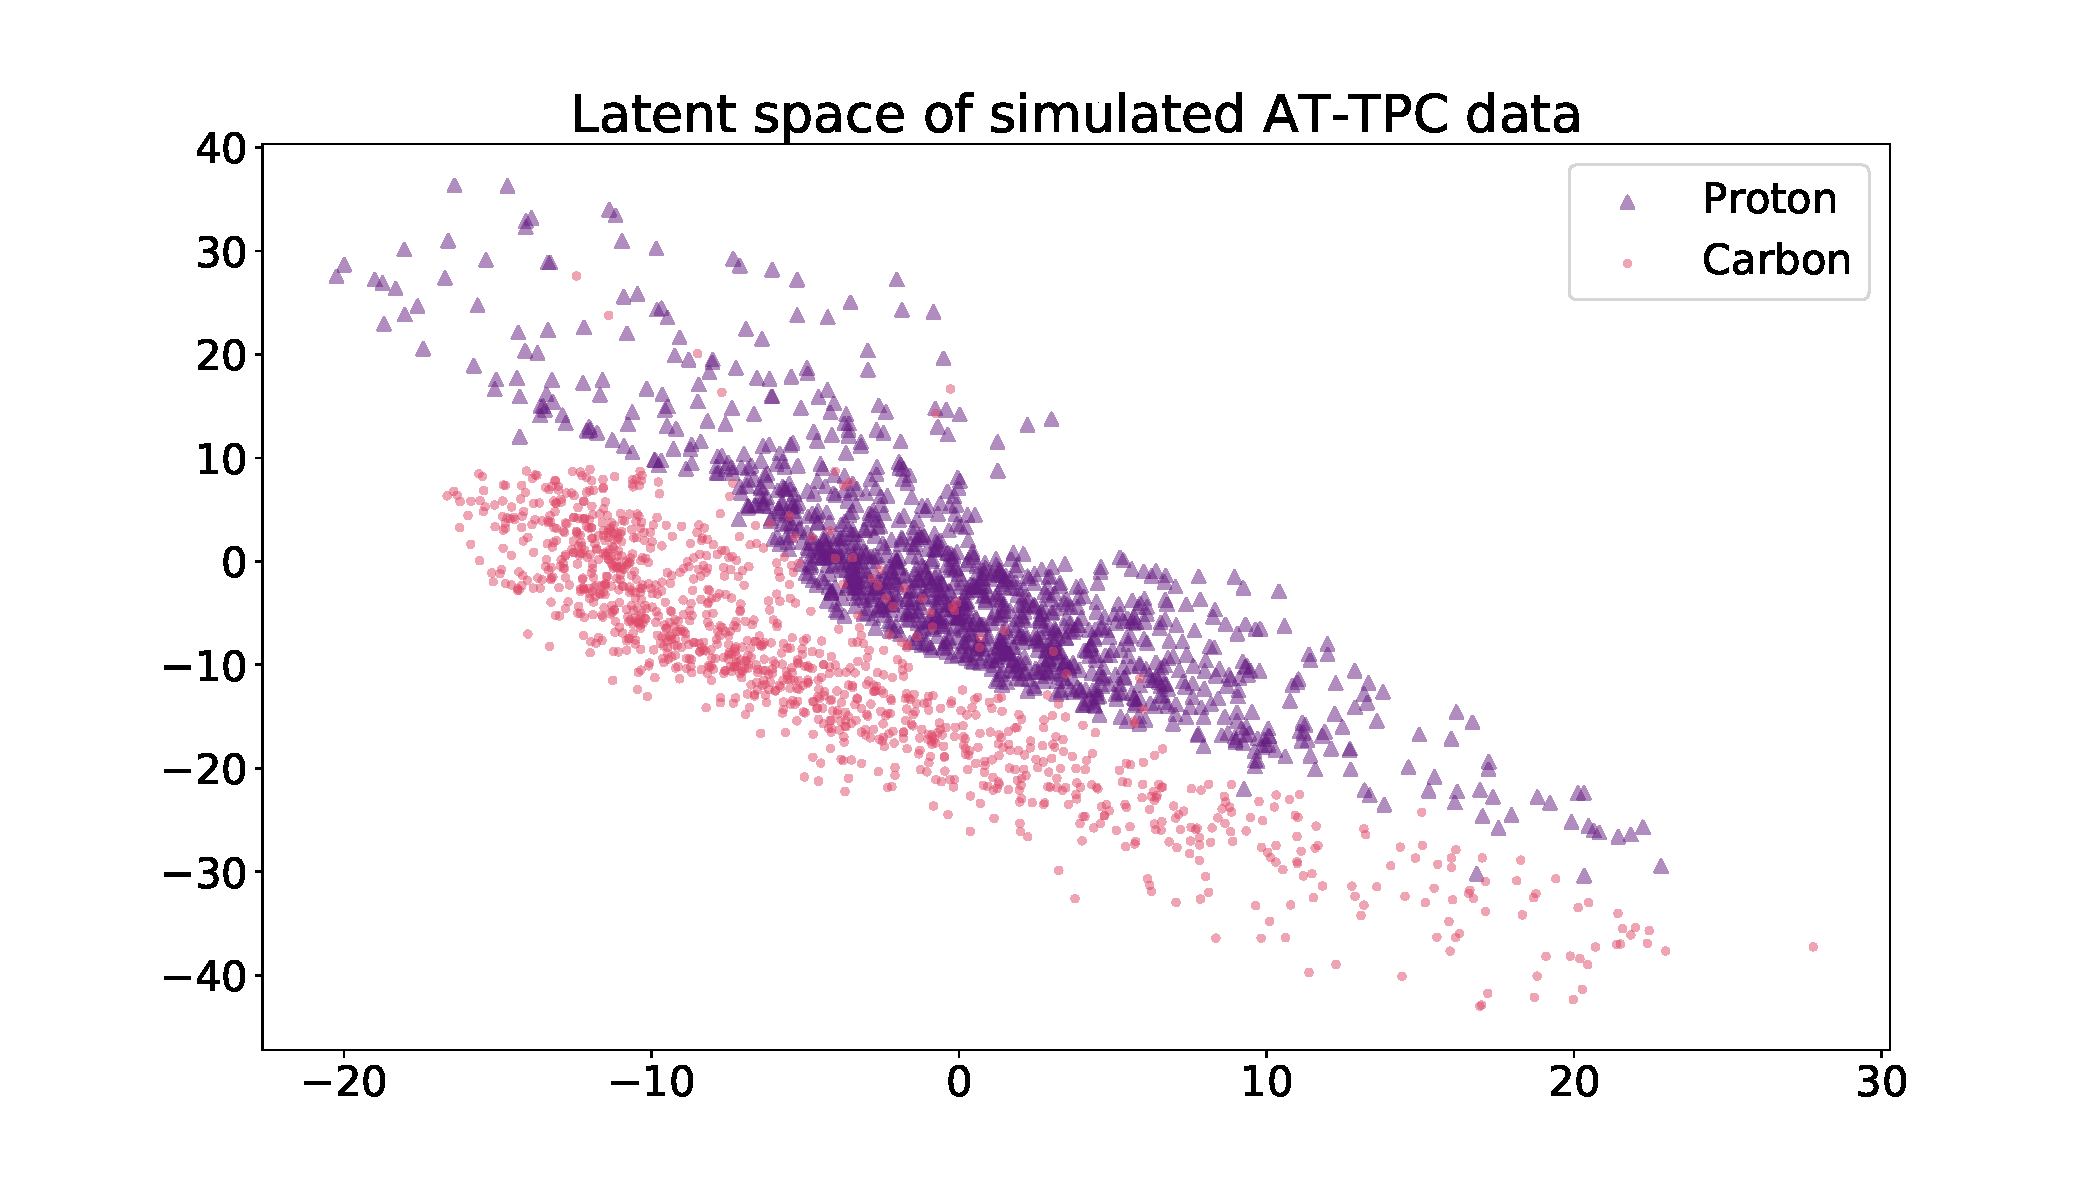
\includegraphics[width=0.7\textwidth, height=7cm]{latent_sim.pdf}
\caption[2D latent space for simulated data]{2D latent space representation of the simulated AT-TPC data.}\label{fig:latent_sim}
\end{figure}

\noindent We visually confirm that the resulting latent space shown in figure \ref{fig:latent_sim} is clearly linearly separable.

